\documentclass[11pt]{beamer}

\usetheme{metropolis}

\usepackage{graphicx}
\usepackage{physics}
\usepackage{adjustbox}
\usepackage{caption}
\usepackage{chemformula}
\usepackage{quoting}
\usepackage[style=chem-angew,backend=bibtex]{biblatex}
\bibliography{references}
%
% Choose how your presentation looks.
%
% For more themes, color themes and font themes, see:
% http://deic.uab.es/~iblanes/beamer_gallery/index_by_theme.html
%
\mode<presentation>
{
  \usetheme{default}      % or try Darmstadt, Madrid, Warsaw, ...
  \usecolortheme{default} % or try albatross, beaver, crane, ...
  \usefonttheme{default}  % or try serif, structurebold, ...
  \setbeamertemplate{navigation symbols}{}
  \setbeamertemplate{caption}[numbered]
  \setbeamerfont{footnote}{size=\tiny}
} 

\usepackage[english]{babel}
\usepackage[utf8]{inputenc}
\graphicspath{{image/}}

\AtBeginSection[]{
\begin{frame}{Outline}
  \tableofcontents[currentsection]
\end{frame}
}

\title{Chapter 5: Chemical Reactions and Equations}
\institute{Chemistry Department, Cypress College}
\date{September 26, 2022}

\begin{document}

\begin{frame}
  \titlepage
\end{frame}

\begin{frame}{Class Announcements}
  \textbf{Lab Section}
  \begin{itemize}
  \item Read the Exp 7: Water in Hydrats Lab
  \item Bunsen burner to heat the hydrate
  \item Temperature change is not required observation
  \item TIP: record all qualitative and quantitative observations
  \end{itemize}

  \textbf{Lecture Section}
  \begin{itemize}
  \item All assignments have been graded
  \item 1.5 hrs Ch. $1 - 4$ exam, questions are based on the lectures,
    homework, and worksheets
  \item Review Ch. 4 material and begin Ch.5 - Chem Reactions and Equations
  \end{itemize}
\end{frame}

\section{Review: Mass Percent, Moles, and Molarity}

\begin{frame}{Elemental Composition of a Penny}
  \begin{center}
    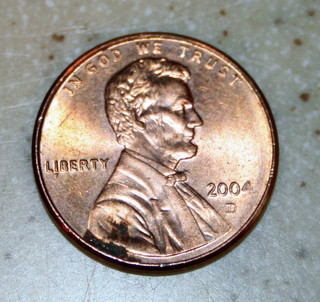
\includegraphics[scale=0.3]{penny_2004}
  \end{center}

  \begin{itemize}
  \item Penny has not been made of solid copper
  \item Mix of cheaper metal along with copper on the surface
  \item Made of $97.5\%$ zinc and $2.5\%$ copper
  \end{itemize}
\end{frame}

\begin{frame}{Different Types of Steel}
  \begin{center}
    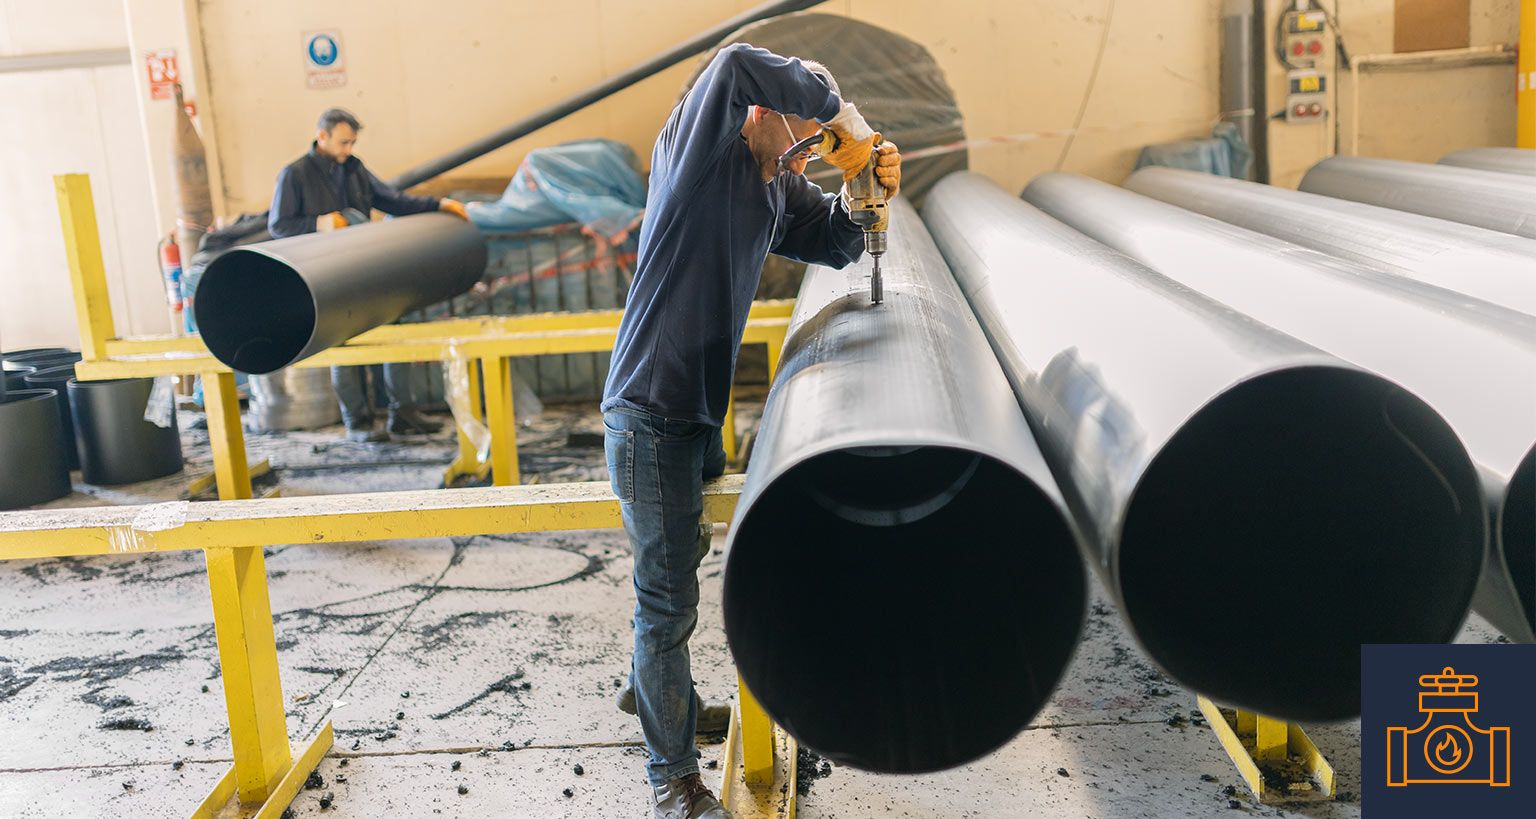
\includegraphics[scale=0.12]{steel_type}
  \end{center}

  \begin{itemize}
  \item Steel is a metal alloy; mixture of different
    metals yield different physical properties
  \item Different types:
    \begin{itemize}
    \item Carbon steel
    \item Stainless steel
    \item Alloy steel
    \item Tool steel
    \end{itemize}
  \end{itemize}
\end{frame}

\begin{frame}{Mass Percent Composition}
  \textbf{Main Takeaway:} Convert the mass of each component
  to a percentage of the total mass

  \begin{equation}
    P_A = \frac{M_A}{M_\text{Tot}} \times 100\%
  \end{equation}

  where $M_\text{Tot}$ is the total mass, $M_A$ is the mass and $P_A$
  is the percent composition for component $A$  
\end{frame}

\begin{frame}{The Mole Concept}
  \begin{center}
    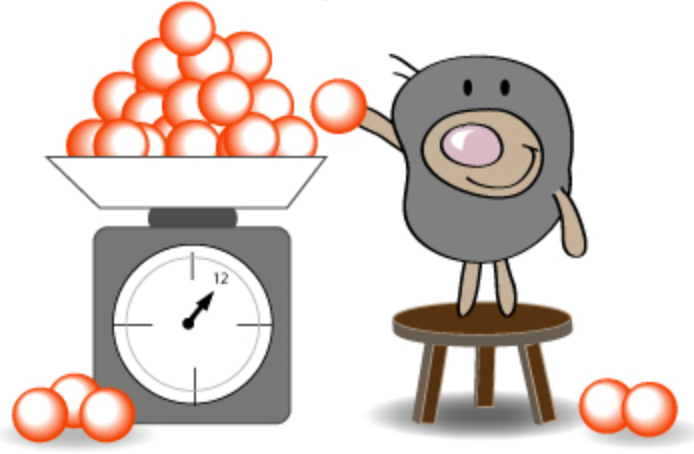
\includegraphics[scale=0.2]{mole}
  \end{center}
  
  \textbf{Q:} What is a mole (mol)?

  \textbf{A:} A mole is measurement of a substance and relates to
  Avogadro's number ($6.022 \times 10^{23}$ molecules/mol)

  \textbf{side note:} Mole day is Oct. 23, between 6:02 a.m. and 6:02 p.m
\end{frame}

\begin{frame}{Purpose of the Mole}
  \begin{center}
    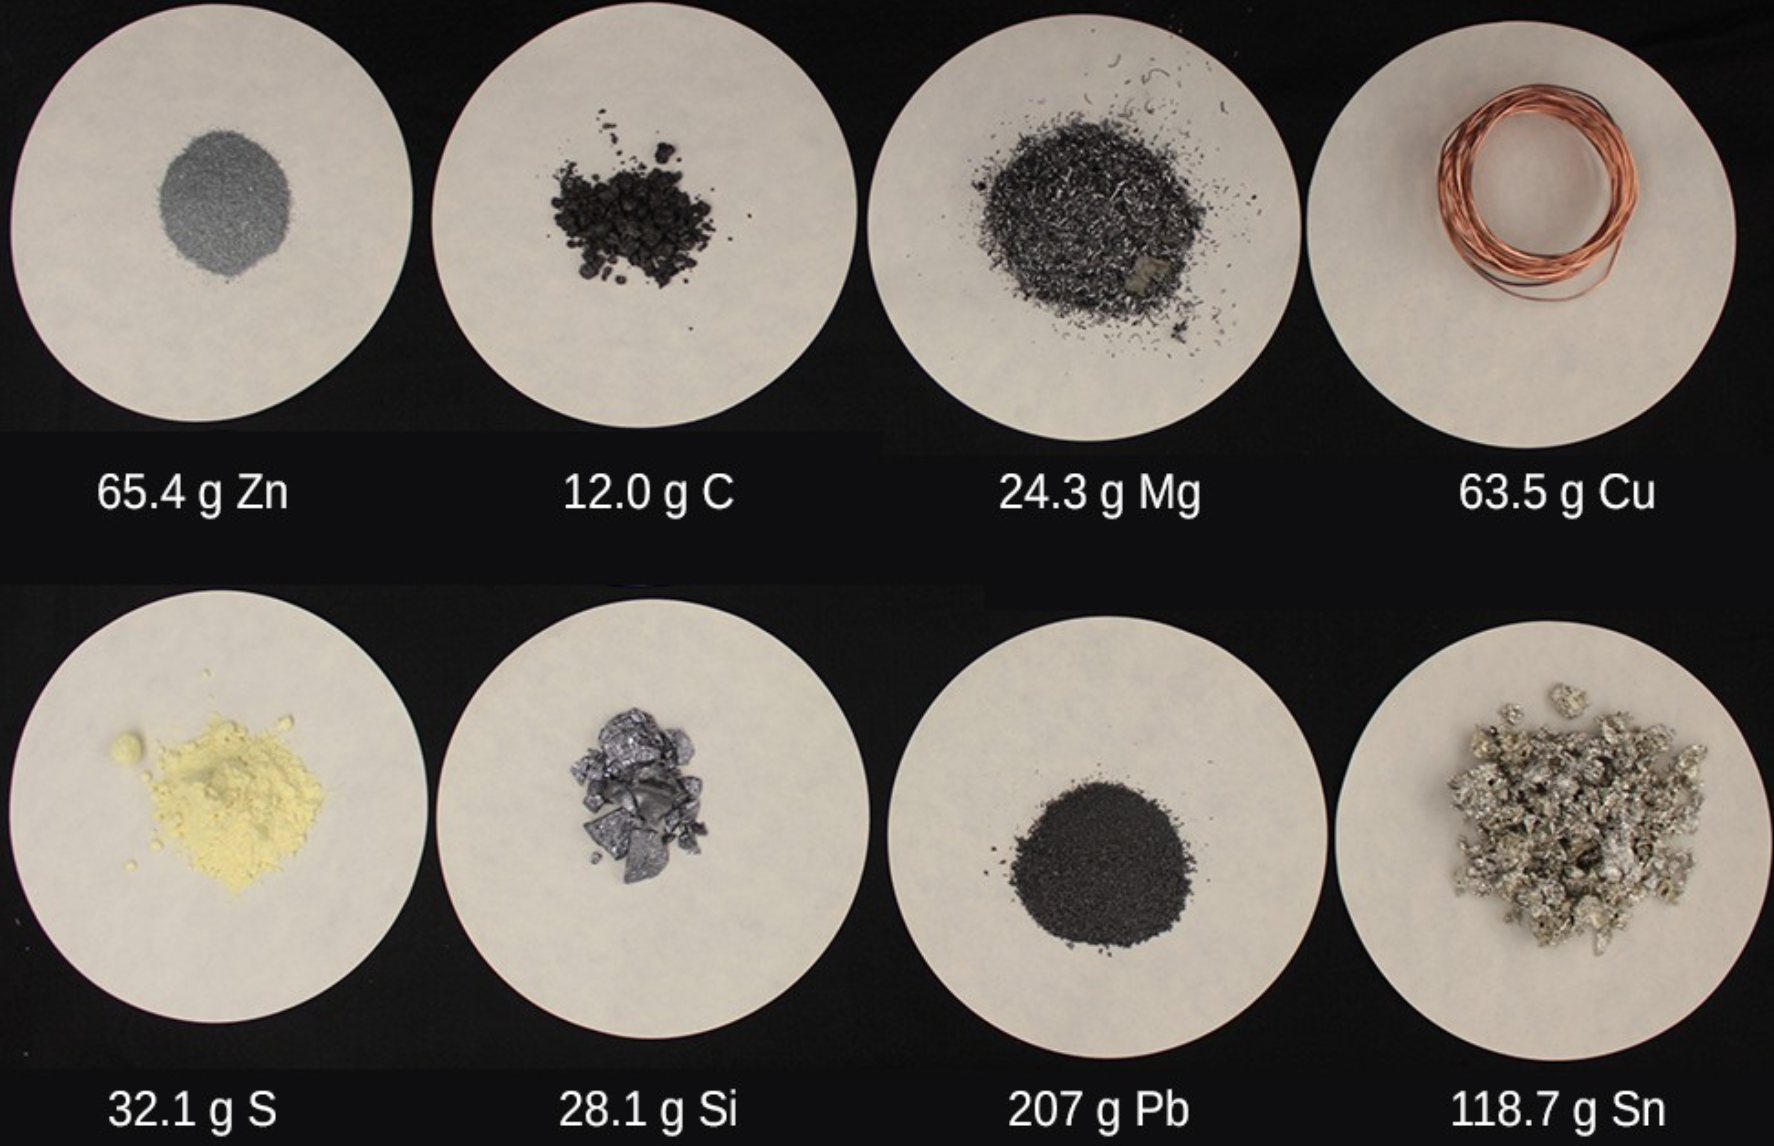
\includegraphics[scale=0.1]{mol_solids}
  \end{center}
  
  \begin{itemize}
  \item Gives a consistent method to convert between atoms/molecules and grams
  \item Convenient way to preform calculations
  \item View the mole (mol) as a unit conversion type approach
  \end{itemize}
\end{frame}

\begin{frame}{Periodic Table Revisited}
  \centering
  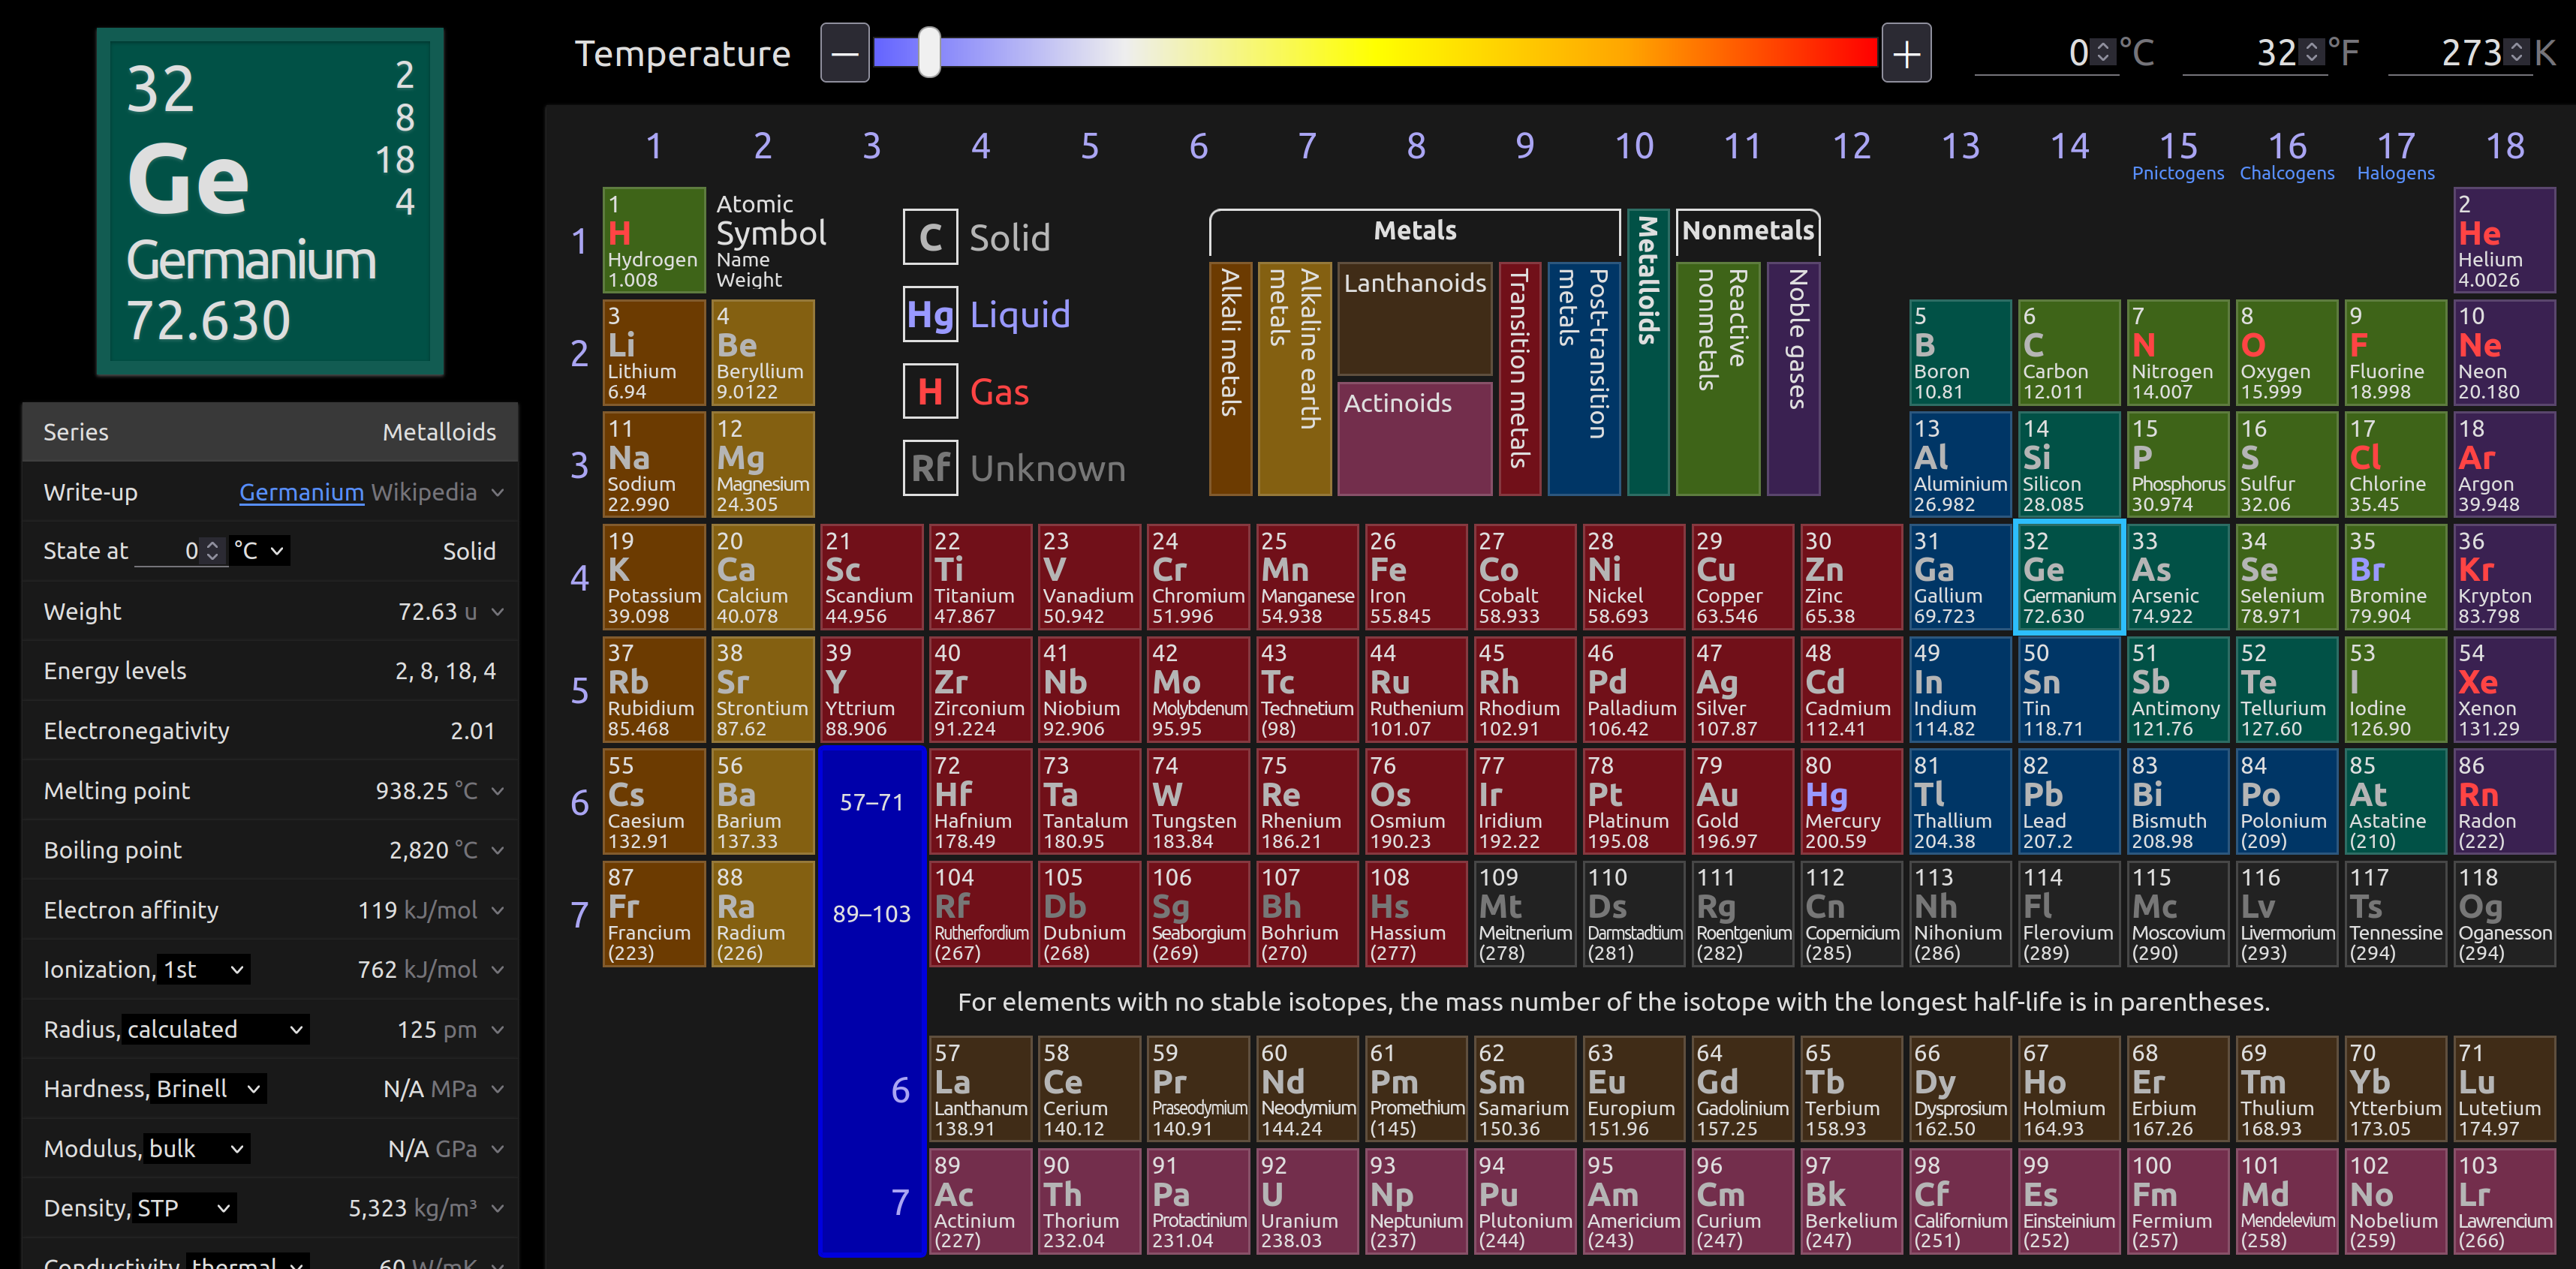
\includegraphics[width=\linewidth]{ptable}

  \textbf{Ge} - 72.630 amu for 1 atom and the molar mass is 72.630 g/mol

  1 amu = $1.66054\times 10^{-24}$ g
\end{frame}

\begin{frame}{Defn: Solvent and Solute}
  \begin{center}
    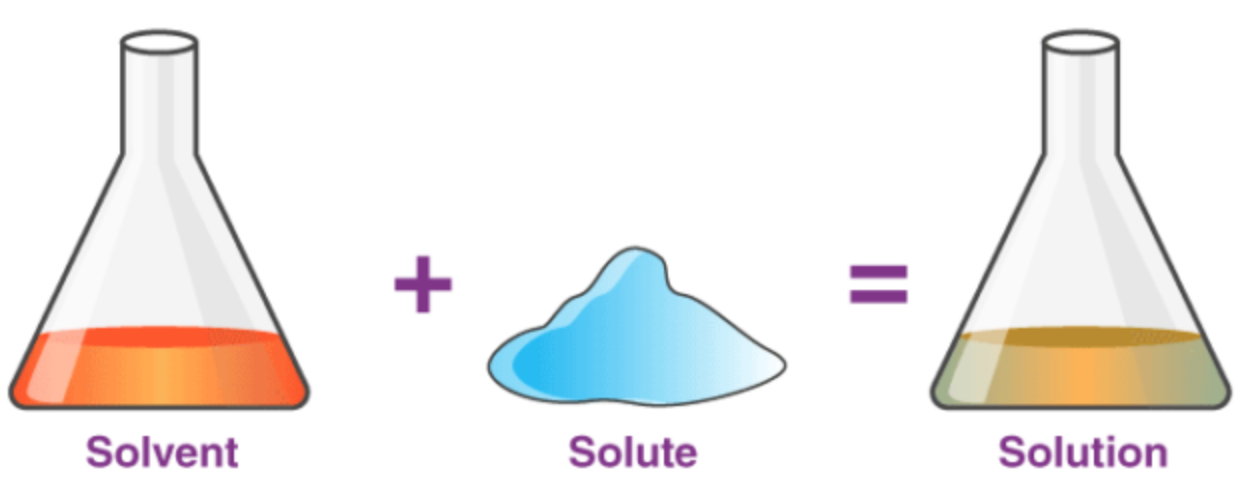
\includegraphics[width=0.75\linewidth]{solut_solv.png}
  \end{center}

  \textbf{Solute} - a substance (solid, liquid, or gas) dissolved in
  a solvent

  \textbf{Solvent} - the material (liquid or gas) that dissolves the
  solute
\end{frame}

\begin{frame}{Molarity - Concentration of Solution}
  \textbf{Definition of Molarity}
  \begin{align}
    M = \frac{n_\text{solute}}{V}
  \end{align}

  where $M$ is molarity, $n_\text{solute}$ is the mols of solute, and $V$ is volume in L

  \textbf{Q:} What is the units for molarity $M$?
\end{frame}

\begin{frame}{Diluting Solutions}
  \begin{center}
    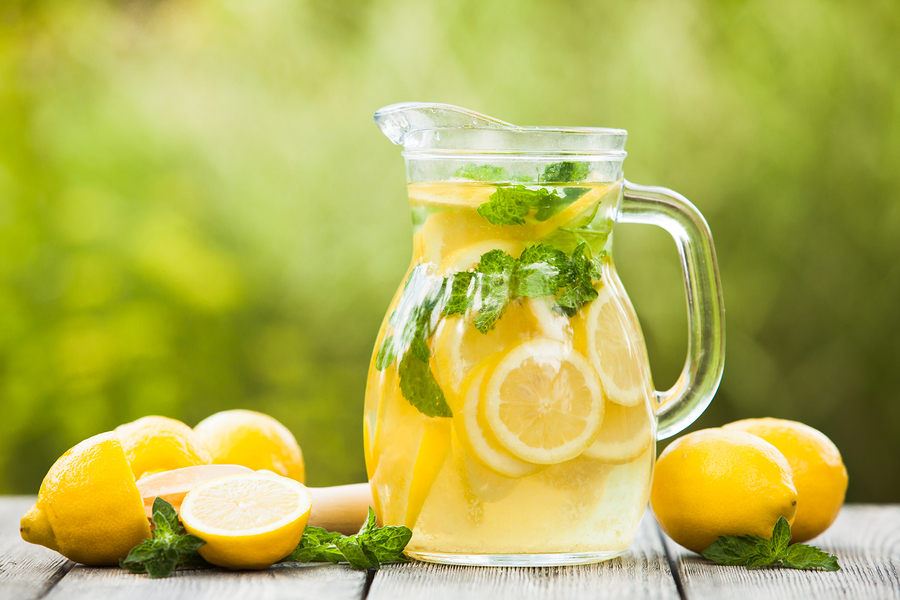
\includegraphics[width=0.4\linewidth]{lemonade}
  \end{center}
  
  Dilution is the process that makes a solution less concentrated. Example is
  lemonade tasting too sweet.

  \textbf{Q:} For given concentrated solution at molarity $M_1$ and a given volume $V_1$, does
  diluting the solution to a new concentration $M_2$ and volume $V_2$ change the amount of mols
  present?
\end{frame}

\section{Chemical Reactions}

\begin{frame}{Chemistry is Everywhere!}
  \centering
  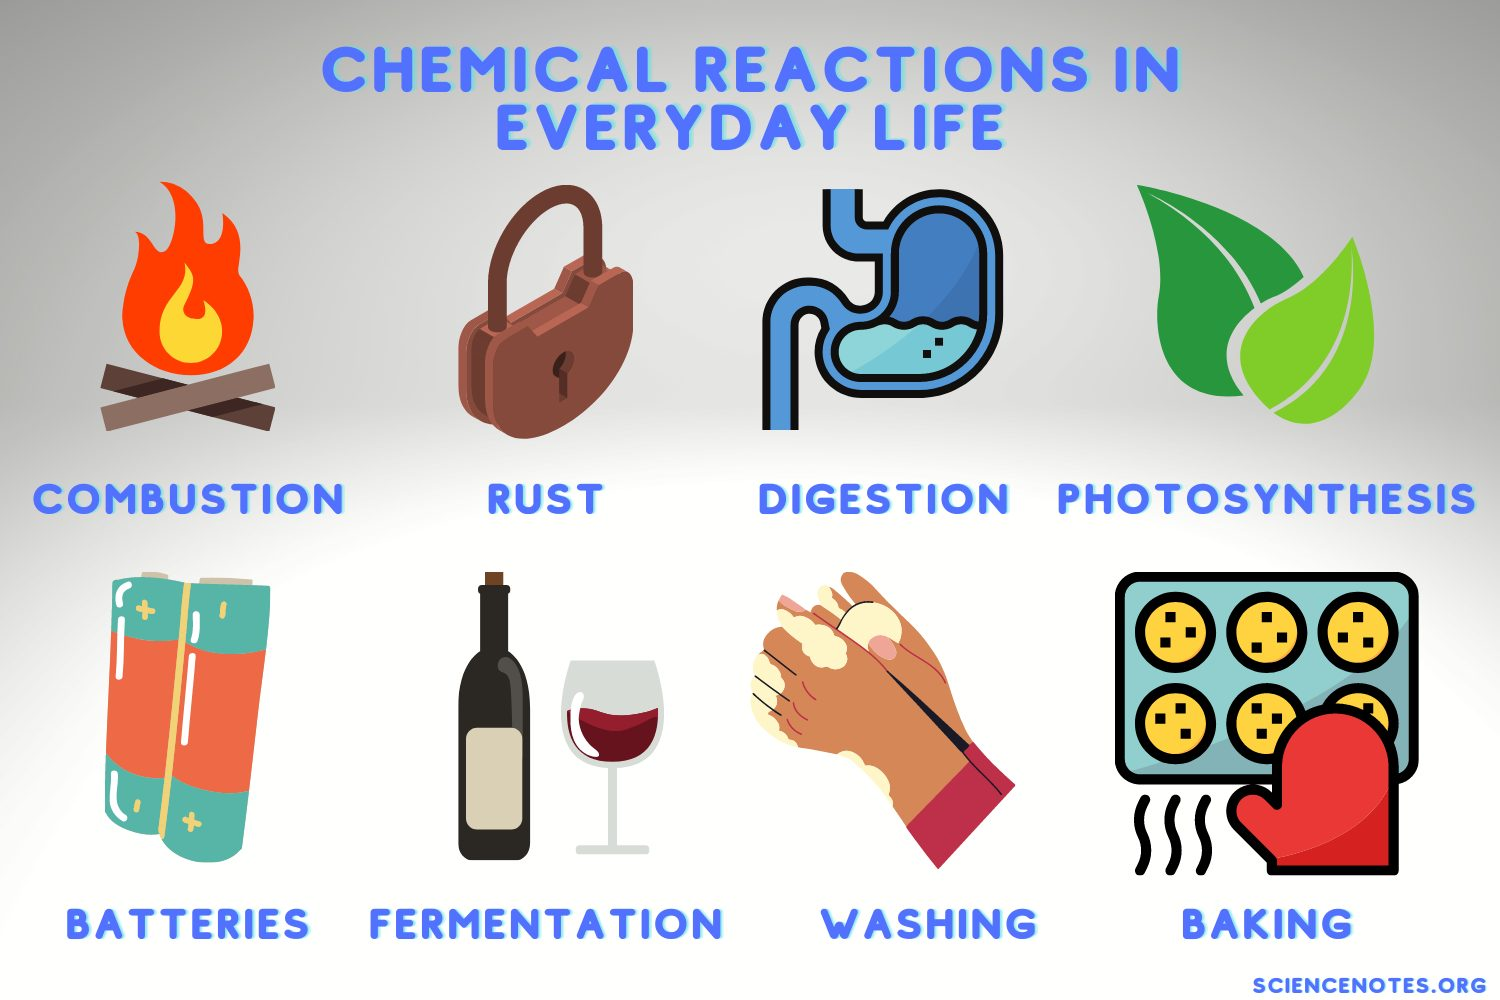
\includegraphics[width=\linewidth]{chem_reactions}
\end{frame}

\subsection{Signs of a Chemical Reaction}

\begin{frame}{Defining a Chemical Reaction}
  \begin{equation}
    A + B \rightarrow C + D
    \label{eqn:chem}
  \end{equation}

  \begin{itemize}
  \item Reactants - chemicals that we start with ($A$ and $B$)
  \item Products - chemicals that are formed after ($C$ and $D$)
    a reaction
  \end{itemize}

  \onslide<2->{\textbf{Q:} Based on Eqn \ref{eqn:chem}, can the reaction go
  in the reverse e.g. $C$ and $D$ turning into $A$ and $B$? Why
  and why not?}
\end{frame}

\begin{frame}{Indications of a Chemical Reaction}
  \begin{center}
    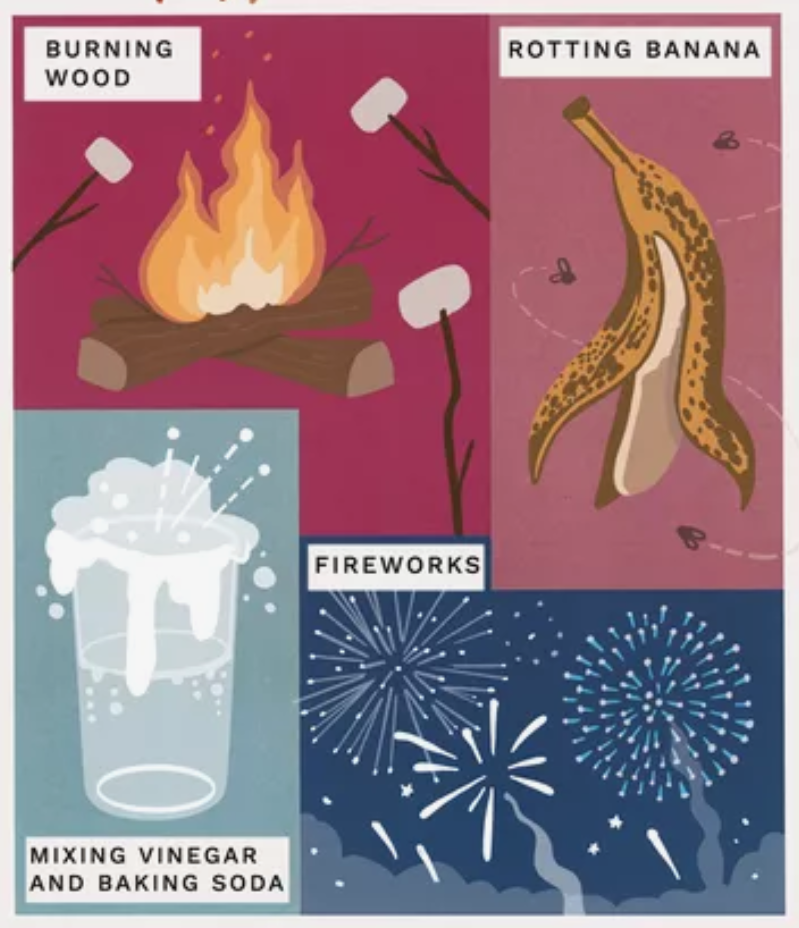
\includegraphics[scale=0.15]{chem_change}
  \end{center}

  \begin{itemize}
  \item Change in color
  \item Production of light
  \item Formation of a solid e.g. precipitate
  \item Formation of a gas
  \item Absorption or release of heat
  \end{itemize}
\end{frame}

\subsection{Writing and Balancing Chem Equations}

\begin{frame}{Writing and Balancing Chem Equations}
  \textbf{Definitions:}

  Chemical equation - symbolic representation of a chemical
  reaction

  Balanced equation - draws upon the conservation of mass; the
  mass of the reactants and the masst of products are equal

  \onslide<2->{\textbf{Q:} Are the moles of reactants and the
    moles of products the same?}
\end{frame}

\begin{frame}{Example: Balancing Chem Equation}
  Balance the following chemical equations:

  \begin{enumerate}[(a)]
  \item CaCl$_2$(aq) + Na$_2$SO$_4$(aq) $\rightarrow$
    CaSO$_4$(s) + NaCl(aq)
  \item[]
  \item CaO(s) + H$_2$O $\rightarrow$ Ca(OH)$_2$(aq)
  \item[]
  \item N$_2$(g) + Mg(s) $\rightarrow$ Mg$_3$N$_2$(s)
  \item[]
  \item CH$_4$(g) + O$_2$(g) $\rightarrow$ CO$_2$(g) + H$_2$O(g)
  \end{enumerate}
  
\end{frame}

\section{Predicting Chemical Reactions}

\subsection{Classes of Reactions}

\begin{frame}{Classes of Reactions}
  \footnotesize
  \begin{table}[hbpt]
    \centering
    \begin{tabular}{c|ccc}
      Class & Reactants & Products & Example \\
      \hline\hline
      Decomposition & 1 compound & multiple   & CD $\rightarrow$ C + D \\
      Combination   & multiple   & 1 compound & A + D $\rightarrow$ AD \\
      Single-displacement & elem+comp & elem+comp & A + CD $\rightarrow$ C +AD\\
      Double-displacement & 2 compounds & 2 compounds & AB + CD $\rightarrow$ AD + BC
    \end{tabular}
  \end{table}
\end{frame}

\begin{frame}{Decomposition Reactions}
\end{frame}

\begin{frame}{Combination Reaction}
\end{frame}

\begin{frame}{Single-Displacement Reaction}
\end{frame}

\begin{frame}{Double-Displacement Reaction}
\end{frame}

\begin{frame}{Example: Chemical Reaction Classifications}
\end{frame}

\subsection{Precipitation Rules}

\begin{frame}{Memorize: Precipitation Rules}
\end{frame}

\begin{frame}{Example:}
\end{frame}

\end{document}
